% Options for packages loaded elsewhere
\PassOptionsToPackage{unicode}{hyperref}
\PassOptionsToPackage{hyphens}{url}
%
\documentclass[
]{article}
\usepackage{amsmath,amssymb}
\usepackage{iftex}
\ifPDFTeX
  \usepackage[T1]{fontenc}
  \usepackage[utf8]{inputenc}
  \usepackage{textcomp} % provide euro and other symbols
\else % if luatex or xetex
  \usepackage{unicode-math} % this also loads fontspec
  \defaultfontfeatures{Scale=MatchLowercase}
  \defaultfontfeatures[\rmfamily]{Ligatures=TeX,Scale=1}
\fi
\usepackage{lmodern}
\ifPDFTeX\else
  % xetex/luatex font selection
\fi
% Use upquote if available, for straight quotes in verbatim environments
\IfFileExists{upquote.sty}{\usepackage{upquote}}{}
\IfFileExists{microtype.sty}{% use microtype if available
  \usepackage[]{microtype}
  \UseMicrotypeSet[protrusion]{basicmath} % disable protrusion for tt fonts
}{}
\makeatletter
\@ifundefined{KOMAClassName}{% if non-KOMA class
  \IfFileExists{parskip.sty}{%
    \usepackage{parskip}
  }{% else
    \setlength{\parindent}{0pt}
    \setlength{\parskip}{6pt plus 2pt minus 1pt}}
}{% if KOMA class
  \KOMAoptions{parskip=half}}
\makeatother
\usepackage{xcolor}
\usepackage{longtable,booktabs,array}
\usepackage{calc} % for calculating minipage widths
% Correct order of tables after \paragraph or \subparagraph
\usepackage{etoolbox}
\makeatletter
\patchcmd\longtable{\par}{\if@noskipsec\mbox{}\fi\par}{}{}
\makeatother
% Allow footnotes in longtable head/foot
\IfFileExists{footnotehyper.sty}{\usepackage{footnotehyper}}{\usepackage{footnote}}
\makesavenoteenv{longtable}
\usepackage{graphicx}
\makeatletter
\def\maxwidth{\ifdim\Gin@nat@width>\linewidth\linewidth\else\Gin@nat@width\fi}
\def\maxheight{\ifdim\Gin@nat@height>\textheight\textheight\else\Gin@nat@height\fi}
\makeatother
% Scale images if necessary, so that they will not overflow the page
% margins by default, and it is still possible to overwrite the defaults
% using explicit options in \includegraphics[width, height, ...]{}
\setkeys{Gin}{width=\maxwidth,height=\maxheight,keepaspectratio}
% Set default figure placement to htbp
\makeatletter
\def\fps@figure{htbp}
\makeatother
\setlength{\emergencystretch}{3em} % prevent overfull lines
\providecommand{\tightlist}{%
  \setlength{\itemsep}{0pt}\setlength{\parskip}{0pt}}
\setcounter{secnumdepth}{-\maxdimen} % remove section numbering
\ifLuaTeX
  \usepackage{selnolig}  % disable illegal ligatures
\fi
\IfFileExists{bookmark.sty}{\usepackage{bookmark}}{\usepackage{hyperref}}
\IfFileExists{xurl.sty}{\usepackage{xurl}}{} % add URL line breaks if available
\urlstyle{same}
\hypersetup{
  hidelinks,
  pdfcreator={LaTeX via pandoc}}

\author{}
\date{}

\begin{document}

\hypertarget{cmpt-276-project---team-meerkat}{%
\section{CMPT 276 Project - Team
Meerkat}\label{cmpt-276-project---team-meerkat}}

\hypertarget{introduction}{%
\subsubsection{Introduction}\label{introduction}}

Welcome to the world of Hive, an intriguing and strategic board game
that will put your tactical skills to the test. In this game, you will
take on the role of a cunning insect monarch, commanding a swarm of
loyal creatures to outmaneuver your opponent and claim dominance over
the Hive.

High-Level Design Choices:

\begin{enumerate}
\def\labelenumi{\arabic{enumi}.}
\item
  Concept: Hive is a two-player, turn-based board game that simulates a
  battle between two colonies of insects. The game board represents a
  hexagonal grid, resembling the layout of a beehive, where players
  strategically place and move their insect tiles.
\item
  Tiles and Abilities: The game consists of different types of insect
  tiles, each with unique abilities and movement patterns. For example,
  the Queen Bee is the most crucial piece, needing to be protected at
  all costs, while other insects like beetles, grasshoppers, ants, and
  spiders possess their own specialized movement abilities.
\item
  Placement and Movement: The game begins with an empty board, and
  players take turns placing their tiles. Once placed, tiles can be
  moved to new positions, but they must always remain connected to the
  hive. Movement options vary for each insect type, allowing for
  strategic positioning and encircling the opponent's pieces.
\item
  Game Objectives: The primary objective is to surround the opponent's
  Queen Bee, effectively trapping it and claiming victory. However,
  there are alternative ways to win, such as capturing the opponent's
  key pieces or forcing their Queen Bee into an immovable position.
\item
  Strategic Depth: While easy to learn, Hive offers a remarkable depth
  of strategy. Planning several moves ahead, anticipating the opponent's
  actions, and adapting to changing situations are key elements for
  success.
\end{enumerate}

In conclusion, Hive is a captivating board game that offers an engaging
and tactical experience for players of all ages. With its unique
insect-themed gameplay, intuitive rules, and depth of strategy, Hive
promises hours of challenging and enjoyable gameplay.

\pagebreak

\hypertarget{architecture}{%
\subsubsection{Architecture}\label{architecture}}

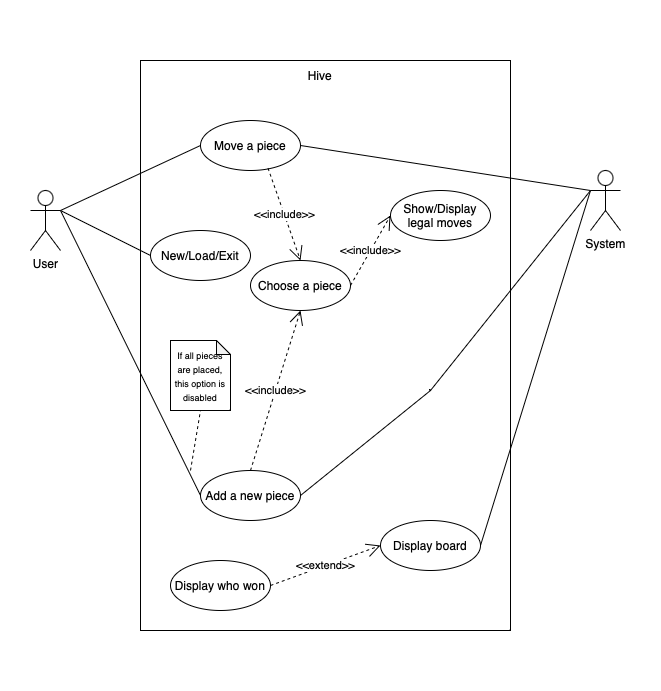
\includegraphics[width=1\textwidth,height=\textheight]{images/hiveusecase.drawio.png}

The implicit hexagonal board used to play Hive requires special
considerations for a proper implementation. Due to the sparse nature and
the possibility of pieces moving indefinitely in any direction,
array-based storage of the board is impractical. We have chosen to use a
map-based storage, indexed by a hexagonal coordinate system. This
coordinate system is derived from a three-dimensional grid of cubes and
was chosen as the coordinates can be added and subtracted without any
special handling.

\begin{figure}
\centering
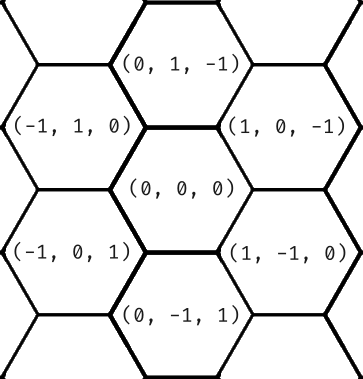
\includegraphics[width=0.5\textwidth,height=\textheight]{images/coords.png}
\caption{The centre of the coordinate grid.}
\end{figure}

Storing the game pieces in a map solves both the issues of the sparse
tiles and the unbounded game field - the amount of memory required is
only proportional the the amount of tiles in play. However, the Beetle
piece provides an additional challenge: multiple pieces can occupy the
same coordinate. This problem is solved by associating each coordinate
with a stack of pieces rather than a single piece.

Each type of piece has different methods of movement, but they are
otherwise identical. As it does not make sense for any piece to inherit
from another, each game piece will inherit from the same abstract class
instead.
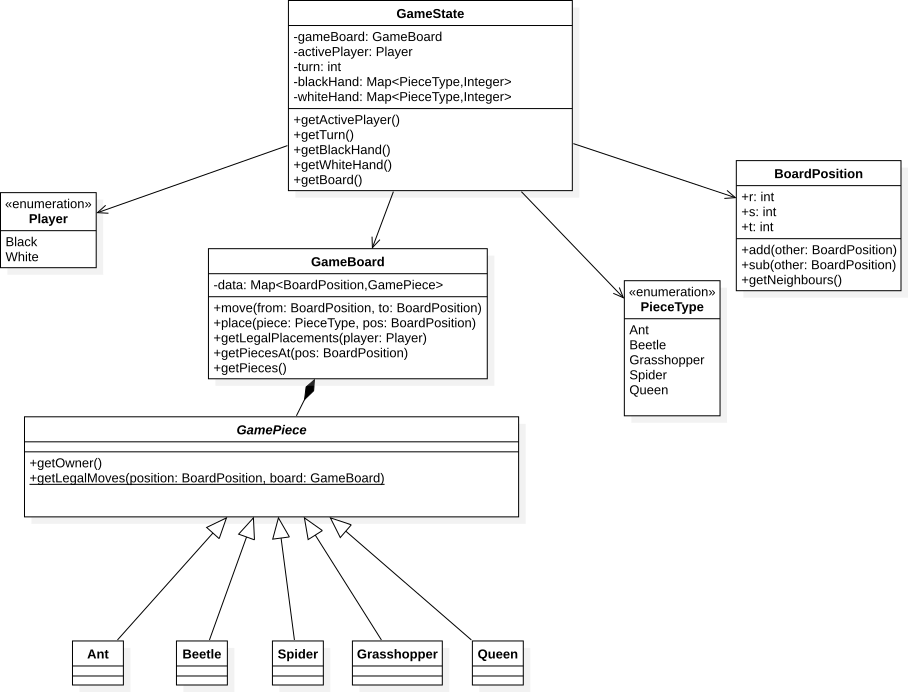
\includegraphics[width=1\textwidth,height=\textheight]{images/class-diag.png}

\hypertarget{user-stories}{%
\subsubsection{User stories}\label{user-stories}}

This game will have two people playing against each other. Each side has
five different characters, Queen Bee, Beetle, Grasshopper, Spider,
Soldier Ant,each insect serves a different purpose.

First, this is the function of each piece. The Queen Bee can move one
space at a time. The Spider must move exactly three spaces per turn. The
Beetle can move one space and also has the ability to climb on top of
other pieces, effectively `pinning' them down. The Grasshopper jumps
over other pieces in a straight line. The Soldier Ant can move around
the hive as far as it wants.

When we start playing this game, the following functions will help us
play Hive very well.

\begin{enumerate}
\def\labelenumi{\arabic{enumi}.}
\item
  Game Pause and Resume: As a player sharing a device with my friend, we
  need to pause our game for a snack break. We tap a new `Pause' button,
  and the game freezes in its current state. When we're ready to
  continue, we tap `Resume', and our game picks up right where we left
  off. This feature helps us maintain our gaming experience despite
  interruptions.
\item
  In-Game Rule Book: As a new player learning to play Hive with my
  friend on the same screen, I'm glad to find an `In-Game Rule Book' in
  the app's menu. This feature lets us quickly refer to the rules and
  piece movements without needing to leave the game or use another
  device. This keeps us focused on enjoying the game and learning as we
  play.
\item
  AI Versus AI Mode: As a player looking to learn more about strategy in
  Hive, I notice a new mode: `AI Versus AI'. I select this mode, and the
  game starts with two AI players facing off. As I watch them play, I
  learn from their strategies and tactics, better preparing me for my
  own games.
\end{enumerate}

\hypertarget{user-story---watch-and-learn-tutorials-learners-perspective}{%
\subsubsection{User Story - Watch and Learn Tutorials (Learner's
perspective):}\label{user-story---watch-and-learn-tutorials-learners-perspective}}

As a new player trying to grasp the basics of Hive, I decide to try the
`Interactive Tutorials'. Instead of just text explanations, the tutorial
starts an AI versus AI game and narrates the strategies and thought
processes behind each move. This interactive and immersive experience
helps me understand the game dynamics much more effectively.

\hypertarget{user-story---save-and-load-games-friends-perspective}{%
\subsubsection{User Story - Save and Load Games (Friend's
perspective):}\label{user-story---save-and-load-games-friends-perspective}}

As a player who often plays long games with my friend on the same
device, I'm thrilled to discover a new `Save Game' feature. Now, when we
have to stop playing, we can save our game state and resume from exactly
where we left off next time.

\hypertarget{user-story---customization}{%
\subsubsection{User Story -
Customization:}\label{user-story---customization}}

Mergatroid Hooperbag, a passionate and enthusiastic player, has just
discovered Hive game -- a game known for its strategic and insects-theme
pieces. She is captivated to the game's strategic depth and the tactile
beauty of the pieces, but she yearns for a personalized gaming
experience comparing to other board games like chess. With the Hive
game's customization system, she finds her needs met. She is given
choices to customise her gameplay as soon as she starts the game,
including the ability to change the board's theme and the colour and
style of her bug pieces. This allows Mergatroid to immerse herself in a
game that feels like her own, tailored to her visual preferences.

\hypertarget{user-story---undo}{%
\subsubsection{User Story - Undo:}\label{user-story---undo}}

Fartbuns Beeman is an experienced player in Hive, but occasionally makes
a mistake because of the complex strategy. On a beautiful Saturday
evening, he is practicing in a tough match against the AI. Suddenly, he
realizes he's made a potentially game-losing mistake by placing his ant
in the wrong spot. But Hive has an undo feature. With a click, he
retracts his move, revaluates his strategy, and continues the match, a
crisis averted and his enjoyment of the game uninterrupted.

\hypertarget{user-story---tutorial}{%
\subsubsection{User Story - Tutorial:}\label{user-story---tutorial}}

The game's distinctive, bug-themed gameplay intrigues Crapps Kingfish, a
rookie to Hive, but he finds the rules to be a little intimidating. On a
beautiful Sunday afternoon, he fires up the game, eager to learn but
unsure of where to begin. Thankfully, the game includes a clear and
engaging tutorial. It leads Crapps Kingfish through many scenarios,
demonstrating the special moves of each piece and even providing
tactical guidance. With the aid of the tutorial, he builds
self-assurance and starts to gradually master the game's mechanics,
converting what could have been a frustrating experience into a fun
learning experience.

\newpage

\hypertarget{requirements}{%
\subsubsection{Requirements}\label{requirements}}

\hypertarget{functional-requirements}{%
\subsubsection{Functional requirements:}\label{functional-requirements}}

\begin{longtable}[]{@{}
  >{\raggedright\arraybackslash}p{(\columnwidth - 2\tabcolsep) * \real{0.5000}}
  >{\raggedright\arraybackslash}p{(\columnwidth - 2\tabcolsep) * \real{0.5000}}@{}}
\toprule\noalign{}
\begin{minipage}[b]{\linewidth}\raggedright
REQUIREMENTS
\end{minipage} & \begin{minipage}[b]{\linewidth}\raggedright
DESCRIPTION
\end{minipage} \\
\midrule\noalign{}
\endhead
\bottomrule\noalign{}
\endlastfoot
Game UI & An interactable game interface; enabling users to easily
interact with the game. Players should be able to interact with the game
without any difficulty \\
\midrule
Turn-Based Gameplay & The game should enforce turn-based gameplay,
allowing each player/AI to take their turns alternately \\
\midrule
Moveable Game Pieces & Players and the computer (AI) need to be able to
move the game pieces, sticking to the official Hive game rule \\
\midrule
Valid Movement & The game should validate the moves made by players,
ensuring they follow the movement rules of each piece type \\
\midrule
Game States (Pause/Save/Load) & Game has a functional Pause/Save/Load
states for players, allowing players to save and resume gameplay at
their convenience \\
\midrule
Win/Lose Condition & The game should be able to accurately detect
Win/Lose conditions based on the state of the queen bee piece (i.e.,
whether it is surrounded) \\
\midrule
Game Restart & Players should have the option to restart the game once
it has ended \\
\end{longtable}

\hypertarget{non-functional-requirements}{%
\subsubsection{Non-functional
requirements:}\label{non-functional-requirements}}

\begin{longtable}[]{@{}
  >{\raggedright\arraybackslash}p{(\columnwidth - 2\tabcolsep) * \real{0.5000}}
  >{\raggedright\arraybackslash}p{(\columnwidth - 2\tabcolsep) * \real{0.5000}}@{}}
\toprule\noalign{}
\begin{minipage}[b]{\linewidth}\raggedright
REQUIREMENTS
\end{minipage} & \begin{minipage}[b]{\linewidth}\raggedright
DESCRIPTION
\end{minipage} \\
\midrule\noalign{}
\endhead
\bottomrule\noalign{}
\endlastfoot
Performance & The game should load considerly fast with good latency \\
\midrule
Compatable & The game should be compatible across multiple platforms,
including Windows, Mac, and Linux \\
\midrule
Usability & The user interface should be intuitive and easy to use;
allowing players to understand how to navigate and play the game without
extensive instructions \\
\midrule
Frame Rate (FPS) & The game should has a considerable decent frame rate
to function; providing a smooth and immersive experience for players \\
\midrule
Maintenance & The game's codebase has to be organised and
well-documented in order to make upgrades and bug patches simple \\
\midrule
Rules Enforcement & The game should enforce the rules of Hive,
preventing players from making illegal moves or violating the game's
mechanics \\
\midrule
Error Handling & The game should provide informative error messages and
handle exceptions gracefully, allowing players to understand and recover
from any issues that may arise during gameplay \\
\end{longtable}

\end{document}
